\begin{frame}
\frametitle{Explain Clay GDSM Model.}
here.
\end{frame}

\begin{frame}
  \frametitle{Nested Components}
  The NuclideModel in a Component can be interchangeably represented by any of 
  the four nuclide transport models. 
    \begin{itemize}
      \item Degradation Rate Based Failure Model
      \item Mixed Cell with Degradation, Sorption, Solubility Limitation
      \item Lumped Parameter Model
      \item 1D van Genuchten Advection Dispersion Solution
    \end{itemize}
\end{frame}

\begin{frame}
  \frametitle{Advection Dispersion Equation}
  \footnotesize{
    In a saturated, reducing environment, contaminants are transported by 
    \textbf{dispersion} and \textbf{advection} \cite{schwartz_fundamentals_2003, 
    wang_introduction_1982, van_genuchten_analytical_1982}: 
    \begin{align}
      J &= J_{dis} + J_{adv}\nonumber\\
      &= -\theta(D_{mdis} + \tau D_m)\nabla C + \theta vC\nonumber\\ 
      &= -\theta D\nabla C + \theta vC \nonumber\\ 
      \intertext{which, for uniform flow in $\hat{k}$, is}
      &=\left(-\theta D_{xx} \frac{\partial C}{\partial x}
             \right)\hat{\imath}
             + \left( -\theta D_{yy} \frac{\partial C}{\partial y}
            \right)\hat{\jmath}
            + \left( -\theta D_{zz} \frac{\partial C}{\partial z}
             + \theta v_zC 
            \right)\hat{k},
      \label{unidirflow}
      \intertext{where}
      J_{dis} &= \mbox{ Total Dispersive Mass Flux }[kg/m^2/s]\nonumber\\
      J_{adv} &= \mbox{ Advective Mass Flux }[kg/m^2/s]\nonumber\\
      \tau &= \mbox{ Toruosity }[-] \nonumber\\
      \theta &= \mbox{ Porosity }[\%] \nonumber\\
      D_m &= \mbox{ Molecular diffusion coefficient }[m^2/s]\nonumber\\
      D_{mdis} &= \mbox{ Coefficient of mechanical dispersivity}[m^2/s]\nonumber\\
      D &= \mbox{ Effective Dispersion Coefficient }[m^2/s]\nonumber\\
      C &= \mbox{ Concentration }[kg/m^3]\nonumber\\
      v &= \mbox{ Fluid Velocity in the medium }[m/s].\nonumber
    \end{align}
    }

\end{frame}

\begin{frame}
  \frametitle{Component Interfaces}
  \footnotesize{
Solutions to this equation can be categorized by their boundary conditions and 
those boundary conditions serve as the interfaces between components in the 
Cyder library of nuclide transport models.

  \begin{figure}[htp!]
    \begin{center}
      \def\svgwidth{\textwidth}
      \input{images/flow.eps_tex}
    \end{center}
    \caption{The boundaries between components are robust interfaces defined by 
    Source Term, Dirichlet, Neumann, and Cauchy boundary conditions.}
    \label{fig:flow}
  \end{figure}
  }
\end{frame}

\begin{frame}
\frametitle{Implicit Timestepping}
\footnotesize{Each Component passes some information radially outward to the nested 
Component immediately containing it and some information radially 
inward to the nested Component it contains. 

Mass distribution in Component 0 at time $t_n$ is found from the inner boundary 
condition at time $t_n$ and the outer boundary condition at $t_{n-1}$. Outer 
boundary conditions are solved for numerically at $t_n$.
For each timestep :

\begin{align}
  BC(i, r_o, c_1, t_n) &= f( BC(i, r_i, c_0, t_n), BC(i, r_o, c_1, t_{n-1}) )
  \intertext{where}
  BC  &= \mbox{boundary condition }\nonumber\\
  i &= \mbox{the isotope }\nonumber\\
  r_i &= \mbox{the inner boundary radius } [m]\nonumber\\
  r_o &= \mbox{the outer boundary radius } [m]\nonumber\\
  c_0 &= \mbox{the innermost Component}\nonumber\\
  c_1 &= \mbox{the Component that contains c}_0\nonumber\\
  f &= \mbox{functional form of the contaminant transport algorithm}\nonumber\\
  t_n &= \mbox{timestep n.}\nonumber
\end{align}
}
\end{frame}


\begin{frame}
  \frametitle{Radionuclide Transport: Rate Based Congruent Release}
  \footnotesize{
The implemented model incorporates the source term made available on the inner boundary into its available mass and defines the resulting boundary conditions at the outer boundary as solely a function of the degradation rate of that component.

This results in the following expression for the mass transfer, 
$m_{ij}(t)$, from cell $i$ to cell $j$ at time $t$ :

\begin{align}
  \dot{m}_{ij}(t) &= f_i(\cdots)m_i(t)
  \label{deg_rate_source_cont}
  \intertext{where}
  \dot{m}_{ij} &= \mbox{ the rate of mass transfer from i to j }[kg/s]\nonumber\\
  f_i &= \mbox{ fractional degradation rate in cell i }[1/s] \nonumber\\
  m_i &= \mbox{ mass in cell i }[kg] \nonumber\\
  t &= \mbox{ time  }[s].\nonumber
\end{align}
For a situation as in Cyder and Cyclus, with discrete timesteps, the mass transferred between discrete times $t_{n-1}$ and $t_n$ is a simple linear function of the transfer rate in \eqref{deg_rate_source_cont}, 

\begin{align}
  m_{ij}^n &= \int_{t_{n-1}}^{t_n}\dot{m}_{ij}(t')dt' \nonumber\\
           &= f_i(\cdots)m_i^{n-1}\left(t_n - t_{n-1}\right).
           \label{deg_rate_source_discrete}
\end{align}
}
\end{frame}


\begin{frame}
  \frametitle{Radionuclide Transport: Rate Based Congruent Release}
  \footnotesize{
  \begin{align}
    \intertext{\textbf{Source Term}}
    m_{ij}^n &= f_i(\cdots)m_i^{n-1}\left(t_n - t_{n-1}\right),
    \intertext{\textbf{Dirichlet}}
    C_{ij}^n &= \frac{m_i^n}{V_{vi}} = \frac{\mbox{ solute mass in cell i }}{\mbox{ void volume in cell i}},
    \intertext{\textbf{Neumann}}
    \frac{\partial C}{\partial z}\hat{k}  &=\frac{ \left(\frac{\dot{m}}{\theta_{i0} V_T - C_{1} }\right) }{z_1 - z_0}\hat{k},
  \intertext{\textbf{Cauchy}}
    -\theta_i D_{zz} \frac{ \left(\frac{\dot{m}}{\theta_{i0} V_T - C_{1} 
  }\right) }{z_1 - z_0}\hat{k} + \theta_i^n v_z^n C_i^n \hat{k}&= \theta_i^{n-1} 
  v_z^{n-1} C_i^{n-1}\hat{k}
    \intertext{where}
    D_{zz} &= \mbox{ $\hat{k}$ component diffusion tensor component in $\hat{k}$ direction }[m^2/s] \nonumber\\
    C_i &= \mbox{ concentration in cell i }[kg/m^3].\nonumber\\
    \theta_i &= \mbox{ porosity in cell i }[-]. \nonumber
  \end{align}
  }
\end{frame}

\begin{frame}
  \frametitle{Radionuclide Transport : Mixed Cell with Sorption and Solubility}
  \footnotesize{
  % Waste Form
  \begin{columns}[c]
  \column{0.45\textwidth}
Before degradation, the volume of the intact matrix can be expressed as
\begin{align}
V_{im}(t_n) &= V_T.
\end{align}

The volume of free fluid can be expressed as
\begin{align}
V_{ff}(t_n) &= \theta V_T .
\end{align}

  \column{0.55\textwidth}
  \begin{figure}[h!]
    \begin{center}
      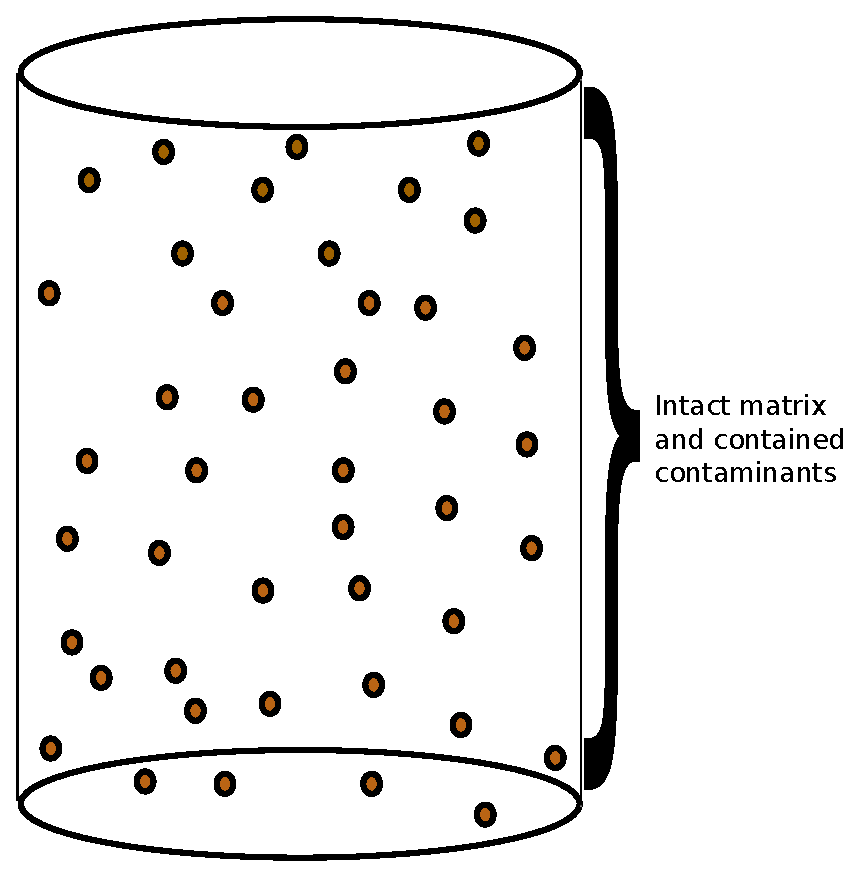
\includegraphics[width=\textwidth]{images/mixed_cell_whole.eps}
    \end{center}
  \end{figure}
\end{columns}
    }
\end{frame}

\begin{frame}[ctb!]
  \frametitle{Radionuclide Transport : Mixed Cell with Sorption and Solubility}
  % Waste Form
  \footnotesize{
  \begin{columns}[c]
  \column{0.45\textwidth}
After some time degrading, the volume of the intact matrix can be expressed as
\begin{align}
V_{im}(t_n) &= V_T - V_T\int_{t_0}^{t_n} f(\cdots) dt.
\label{vim}
\end{align}

The volume of free fluid can be expressed as
\begin{align}
V_{ff}(t_n) &= \theta V_T \int_{t_0}^{t_n} f(\cdots) dt.
\label{vff}
\end{align}

Finally, the volume of the degraded and precipitated solids can be expressed as
\begin{align}
V_{ps}(t_n) &= (1 - \theta)V_T\int_{t_0}^{t_n} f(\cdots) dt.
\label{vps} 
\end{align}
 

\column{0.55\textwidth}
  \begin{figure}[h!]
    \begin{center}
      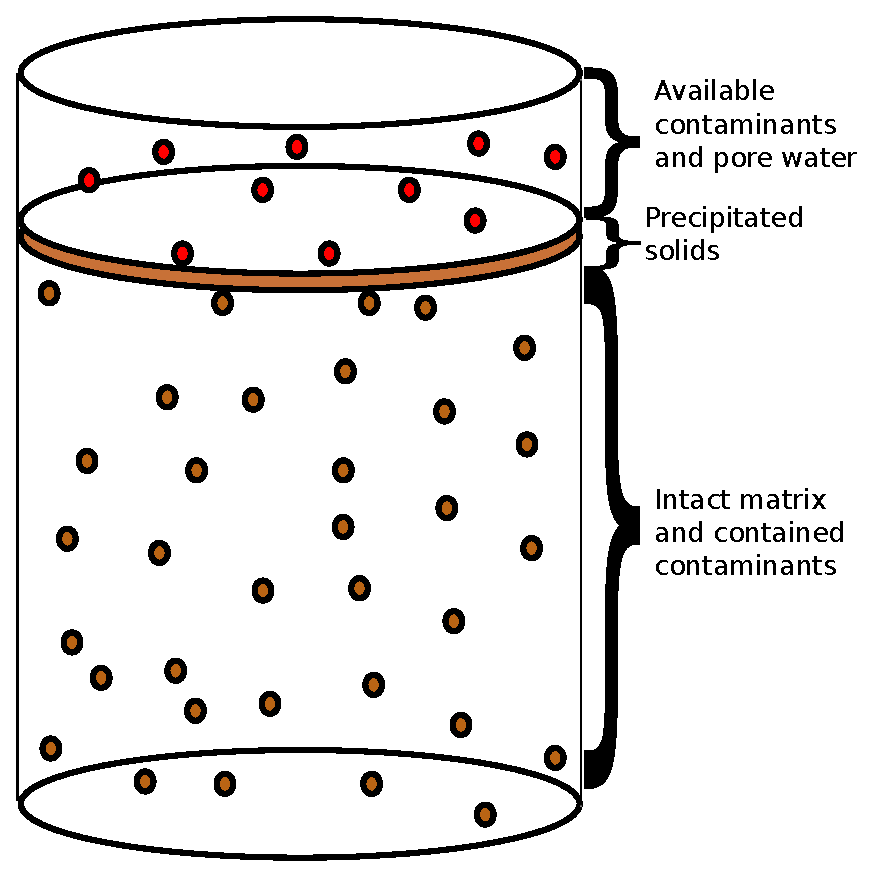
\includegraphics[width=\textwidth]{images/mixed_cell_degraded.eps}
    \end{center}
  \end{figure}
\end{columns}
}
\end{frame}

\begin{frame}
  \frametitle{Radionuclide Transport : Mixed Cell Sorption}
  \footnotesize{

The mass of contaminant sorbed into the degraded and precipitated solids can be
found using a linear isotherm model \cite{schwartz_fundamentals_2003},
characterized by the relationship 
\begin{align}
s_{i} &= K_{di} c_{i}
\label{linear_iso}
\intertext{where}
s_i &= \mbox{ the solid concentration of isotope i }[kg/kg]\nonumber\\
K_{di} &= \mbox{ the distribution coefficient of isotope i}[m^3/kg]\nonumber\\
c_i &= \mbox{ the liquid concentration of isotope i }[kg/m^3].\nonumber
\end{align}

From the sorbed contaminant mass, we find the non-sorbed contaminant mass in the free fluid,

\begin{align}
m_{ffl}   &= m_{ffT} - \frac{1}{2} \left(m_{ffT} - m_{psm} - \frac{V_{ff}}{K_d}\right) \nonumber\\
          & \mp \frac{1}{2} \sqrt{m_{ffT}^2 + 2m_{ffT}\left(m_{psm} - 
          \frac{V_{ff}}{K_d}\right) + \left(m_{psm} + 
          \frac{V_{ff}}{K_d}\right)^2}.
\label{m_ffl_full}
\intertext{where}
m_{ffT}  &= \mbox{ total degraded contaminant mass }[kg]\nonumber\\
m_{psm}  &= \mbox{ noncontaminant mass in degraded and precipitated solids }[kg]\nonumber\\
m_{psc}  &= \mbox{ contaminant mass in degraded and precipitated solids }[kg]\nonumber\\
\rho_b   &= \mbox{ bulk (dry) density of the medium }[kg/m^3].\nonumber\\
\end{align}

    }
\end{frame}

\begin{frame}[ctb]
\frametitle{Radionuclide Transport: Retardation Sensitivity Expected Behavior}
\begin{figure}[ht]
  \centering
  \includegraphics[height=60mm]{images/Partitioning_Summary.eps}
  \caption{Generated with the Used Fuel Disposition Campaign's Generic Disposal 
  System Model for Clay, this graph demonstrates $K_d$ sensitivity. 
  The peak annual dose due to an inventory, $N$, of each isotope.}
  \label{fig:KdSum}
\end{figure}
\end{frame}


\begin{frame}
  \frametitle{Radionuclide Transport : Mixed Cell Solubility Limitation}
  \footnotesize{
In addition to engineered barriers, contaminant transport is constrained by 
  the solubility limit \cite{hedin_integrated_2002}, 
    \begin{align}
      m_{s,i} &\leq V_w C_{sol,i},
    \intertext{where}
      m_{s,i} &= \mbox{ solubility limited mass of isotope i in volume }V_w [kg]\nonumber\\ 
      V_w &= \mbox{ volume of the solution }[m^3]\nonumber\\
      C_{sol,i} &= \mbox{ solubility limit, the maximum concentration of i }[kg/m^3].\nonumber
    \end{align}


The desired boundary conditions can be expressed in terms of $m_{ffl}$. First, the 
Dirichlet boundary condition is 
\begin{align}
C(x,y,z,t) = \frac{m_{ffl}(t)}{V_{ff}(t)}\forall (x,y,x) \in \Gamma.
\label{dirichlet_mixed}
\end{align}

From this boundary condition in combination with global advective velocity 
data, all other boundary conditions can be found. 
    }
\end{frame}

\begin{frame}[ctb]
\frametitle{Radionuclide Transport: Solubility Sensitivity Expected Behavior}
\begin{figure}[ht]
  \centering
  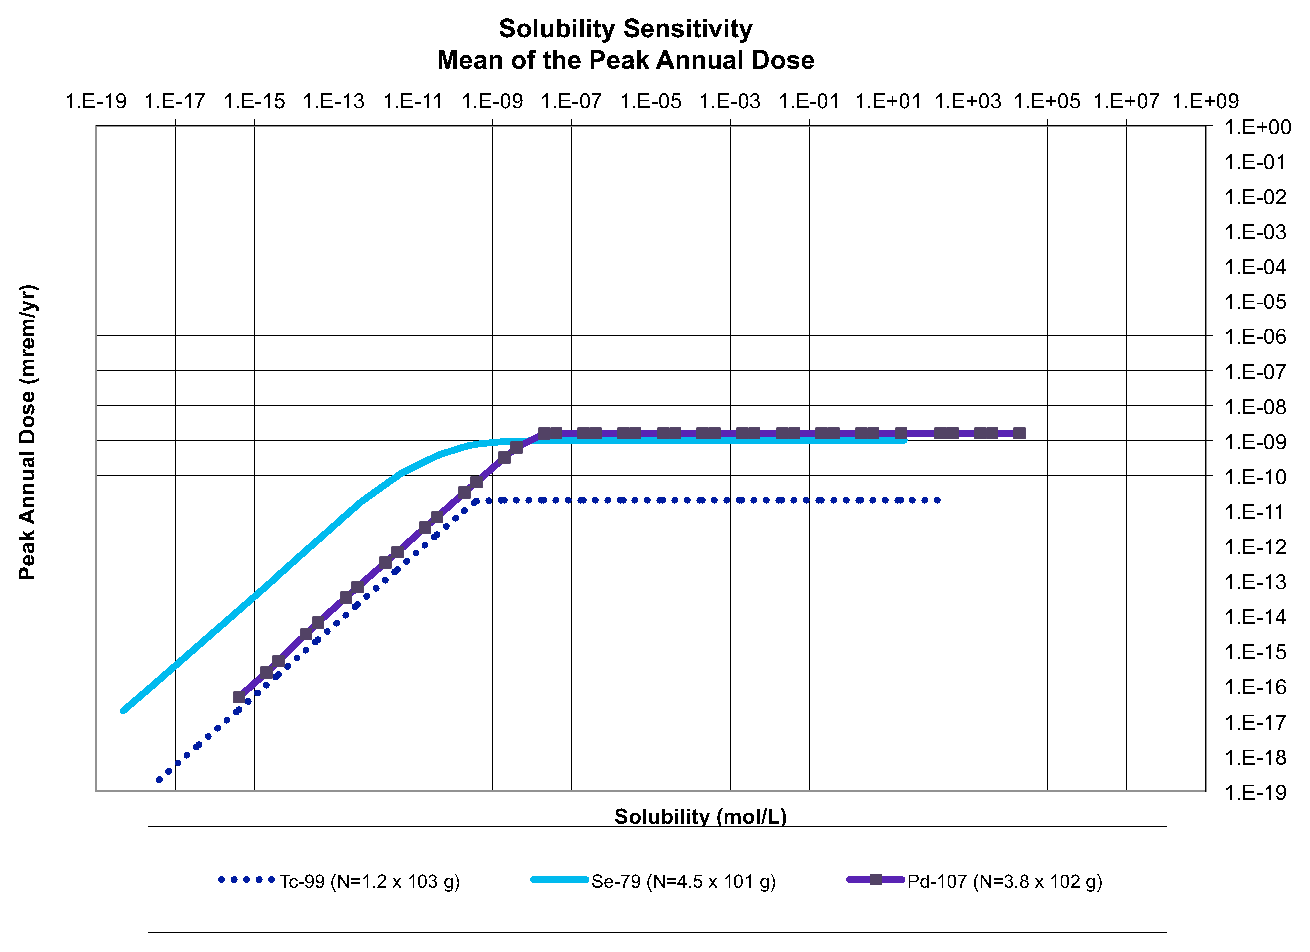
\includegraphics[height=60mm]{images/Solubility_Summary.eps}
  \caption{Generated with the Used Fuel Disposition Campaign's Generic Disposal 
  System Model for Clay, this graph demonstrates solubility limit sensitivity. 
  The peak annual dose due to an inventory, $N$, of each isotope.}
  \label{fig:SolSum}
\end{figure}
\end{frame}


\begin{frame}
  \frametitle{Radionuclide Transport: Lumped Parameter Transport Model}
\footnotesize{
\begin{figure}[htbp!]
  \begin{center}
    \def\svgwidth{\textwidth}
    \input{images/lumpedseries.eps_tex}
  \end{center}
  \caption{ The method by which each lumped parameter component is modeled is
according to a relationship between the incoming concentration, $C_{in}(t)$,
and the outgoing concentration, $C_{out}(t)$.}
  \label{fig:lumpedseries}
\end{figure}

\begin{align}
  C_{out}(t) &= \int_0^\infty C_{in}(t-t')g(t')e^{-\lambda t'}dt'
  \label{lumped2}
  \intertext{where}
  t'  &= \mbox{ time of entry }[s]\nonumber\\
  t-t'  &= \mbox{ transit time }[s]\nonumber\\
  g(t-t')  &= \mbox{ response function, a.k.a. transit time distribution}[-]\nonumber\\
  \lambda &= \mbox{ radioactive decay constant, 1 to neglect}[s^{-1}].\nonumber
\end{align}
}
\end{frame}

\begin{frame}
  \frametitle{Radionuclide Transport: Lumped Parameter Transport Model}
\footnotesize{
Selection of the response function is usually based on experimental tracer 
results in the medium at hand. However, some functions used commonly in chemical 
engineering applications \cite{maloszewski_lumped_1996} include the Piston Flow 
Model (PFM), Exponential Model (EM), and Dispersion Model (DM),
\begin{align}
  g_{PFM}(t') &= \delta{(t'-t_t))}\\
  g_{EM}(t') &= \frac{1}{t_t}e^{-\frac{t'}{t_t}}\\
  g_{DM}(t') &= \left( \frac{\texttt{Pe }t_t}{4\pi t'} \right)^{\frac{1}{2}}
  \frac{1}{t'}e^{- \frac{\texttt{Pe }t_t\left( 1- \frac{t'}{t_t}  \right)^2} 
  {4t'}}, \intertext{where}
  \texttt{Pe }  &= \mbox{ Peclet number for mass diffusion }[-]\nonumber\\
  t_t  &= \mbox{ mean tracer age }[s]\nonumber\\
       &= \frac{z\theta_e}{q}\nonumber\\
  z    &= \mbox{ average travel distance in flow direction }[m]\nonumber\\
  q    &= \mbox{ Darcy Flux }[m/s]\nonumber\\
  \theta_e &= \mbox{ effective (connected) porosity }[\%].\nonumber
\end{align}
}
\end{frame}

\begin{frame}
  \frametitle{Radionuclide Transport: Lumped Parameter Transport Model}
\footnotesize{
The latter of these, the Dispersion Model satisfies the one dimensional 
advection-dispersion equation, and is therefore the most physically relevant for 
this application. The solutions to these for constant concentration at the 
source boundary are given in \cite{maloszewski_lumped_1996}, 
\begin{align}
  C(t) &=\begin{cases}
    PFM & C_0e^{-\lambda t_t}\\
    EM  & \frac{C_0}{1+\lambda t_t}\\
    DM & C_0e^{\frac{\texttt{Pe}}{2}\left(1-\sqrt{1+\frac{4\lambda 
    t_t}{\texttt{Pe}}}\right)}.
  \end{cases}
  \label{lumpedsolns}
\end{align}
}
\end{frame}


\begin{frame}
  \frametitle{Radionuclide Transport: 1D Semi-Infinite, Cauchy B.C.}
  \footnotesize{
\begin{figure}[htbp!]
  \begin{center}
    \def\svgwidth{.5\textwidth}
    \input{images/1dinf.eps_tex}
  \end{center}
  \caption{A one dimensional, semi-infinite model, unidirectional flow,
  solution with Cauchy and Neumann boundary conditions}
  \label{fig:1dinf}
\end{figure}

The solution is given (van Genuchten et al., \cite{van_genuchten_analytical_1981})  for the
boundary conditions :

For the boundary conditions, 
\begin{align}
  -D \frac{\partial C}{\partial z}\big|_{z=0} + v_zc &= \begin{cases}
    v_zC_0  &  \left( 0<t<t_0 \right)\\
    0  &  \left( t>t_0 \right)\\
  \end{cases},\\
  \frac{\partial C}{\partial z}\big|_{z=\infty} &= 0
  \intertext{and the initial condition,}
  C(z,0) &= C_i.
  \label{1dinfBC}
\end{align}
}
\end{frame}

\begin{frame}[ctb!]
\frametitle{Radionuclide Transport: 1D Semi-Infinite, Cauchy B.C.}
The solution is given (van Genuchten et al., 
\cite{van_genuchten_analytical_1981}) as
\begin{align}
C(z,t) =& \begin{cases} 
  C_0A(z,t) + B(z,t) & 0<t\le t_0\\
  C_0A(z,t) + B(z,t) - C_0A(z,t-t_0)& t\ge t_0
  \end{cases}.
  \label{simple_genuchten}
  \end{align}
\end{frame}

\begin{frame}
\frametitle{Radionuclide Transport: 1D Semi-Infinite, Cauchy B.C.}
\footnotesize{
For the vertical flow coordinate system, $A$ and $B$ are defined as
\begin{align}
A(z,t) =& 
\left(\frac{v}{v+u}\right)\exp{\left[\frac{(v-u)z}{2D}\right]}\erfc{\left[\frac{Rz-ut}{2\sqrt{DRt}}\right]} \nonumber\\
&+ \left(\frac{v}{v-u}\right)\exp{\left[\frac{(v+u)z}{2D}\right]}\erfc{\left[\frac{Rz+ut}{2\sqrt{DRt}}\right]} \nonumber\\ 
&+ \left(\frac{v^2}{2\mu D}\right) \exp{\left[\frac{vz}{D} - \frac{\mu t}{R}\right]}\erfc{\left[\frac{Rz+vt}{2\sqrt{DRt}}\right]}\\
B(z,t) =& 
\left(\frac{\gamma}{\mu} - C_i\right)\Bigg\{ \frac{1}{2}\erfc{\left[\frac{Rz - vt}{2\sqrt{DRt}}\right]}\nonumber\\
&+ \left(\frac{v^2t}{\pi RD}\right)^{1/2}\exp{\left[-\frac{(Rz-vt)^2}{4DRt}\right]}\nonumber\\ 
&- \frac{1}{2} \left(1+\frac{vz}{D} + \frac{v^2t}{DR}\right) \exp{\left[\frac{vz}{D}\right]}\erfc{\left[\frac{Rz+vt}{2\sqrt{DRt}}\right]}\Bigg\}\\
\intertext{where}
u =& v\sqrt{\left(1+\frac{4\mu D}{v^2}\right)}\nonumber\\
R =& \mbox{Retardation factor }[-].\nonumber
\end{align}
}
\end{frame}


\begin{frame}
\frametitle{Radionuclide Transport: 1D Semi-Infinite, Cauchy B.C.}
\footnotesize{
The 1d solution given in van Genuchten et al., \cite{van_genuchten_analytical_1981} is simplified 
with some assumptions. Specifically, in Cyclus, radioactive decay is handled external 
to the components.
\begin{align}
A(z,t) =& 
\left(\frac{1}{2}\right)\erfc{\left[\frac{Rz-vt}{2\sqrt{DRt}}\right]} \nonumber\\
&+ \left(v\infty\right)\exp{\left[\frac{2vz}{2D}\right]}\erfc{ \left[\frac{Rz+vt}{2\sqrt{DRt}}\right]}
\intertext{which remains valid at long distances and times, when }
\left[\frac{Rz+vt}{2\sqrt{DRt}}\right] >> 2
\intertext{such that}
A(z,t) =& 
\left(\frac{1}{2}\right)\erfc{\left[\frac{Rz-vt}{2\sqrt{DRt}}\right]} \\
\end{align}
Finally, simplifying $B(z,t)$ accordingly,
\begin{align}
B(z,t) =& 
\left(- C_i\right)\Bigg\{ \frac{1}{2}\erfc{\left[\frac{Rz - vt}{2\sqrt{DRt}}\right]}\nonumber\\
&+ \left(\frac{v^2t}{\pi RD}\right)^{1/2}\exp{\left[-\frac{(Rz-vt)^2}{4DRt}\right]}\Bigg\}.
  \label{simple_genuchten}
\end{align}
}
\end{frame}
